%!TEX root = main.tex 

\section{Background and Motivation} 
\label{sec:motivation} 

\subsection{Large-scale LLM Training} 
\label{subsec:background}



% Advancements in infrastructure have dramatically increased the scale and complexity of modern AI training. 
\noindent Figure~\ref{fig:tech_overview} illustrates the layered technical stack underlying LLM training, from high-level models and frameworks to low-level GPU libraries and networked systems. 
% Today's LLMs often exceed 100 billion parameters~\cite{jiang2024preventing,llama3-meta}, and recent GPU architectures (e.g., NVIDIA Hopper and Ampere) combined with high-speed interconnects (e.g., InfiniBand and RoCE) enable efficient training at the scale of thousands of GPUs. Parallelism strategies with communication-computation overlap \cite{liu2024deepseek} further improve utilization and accelerate training.

\begin{figure}[t]
    \centering 
    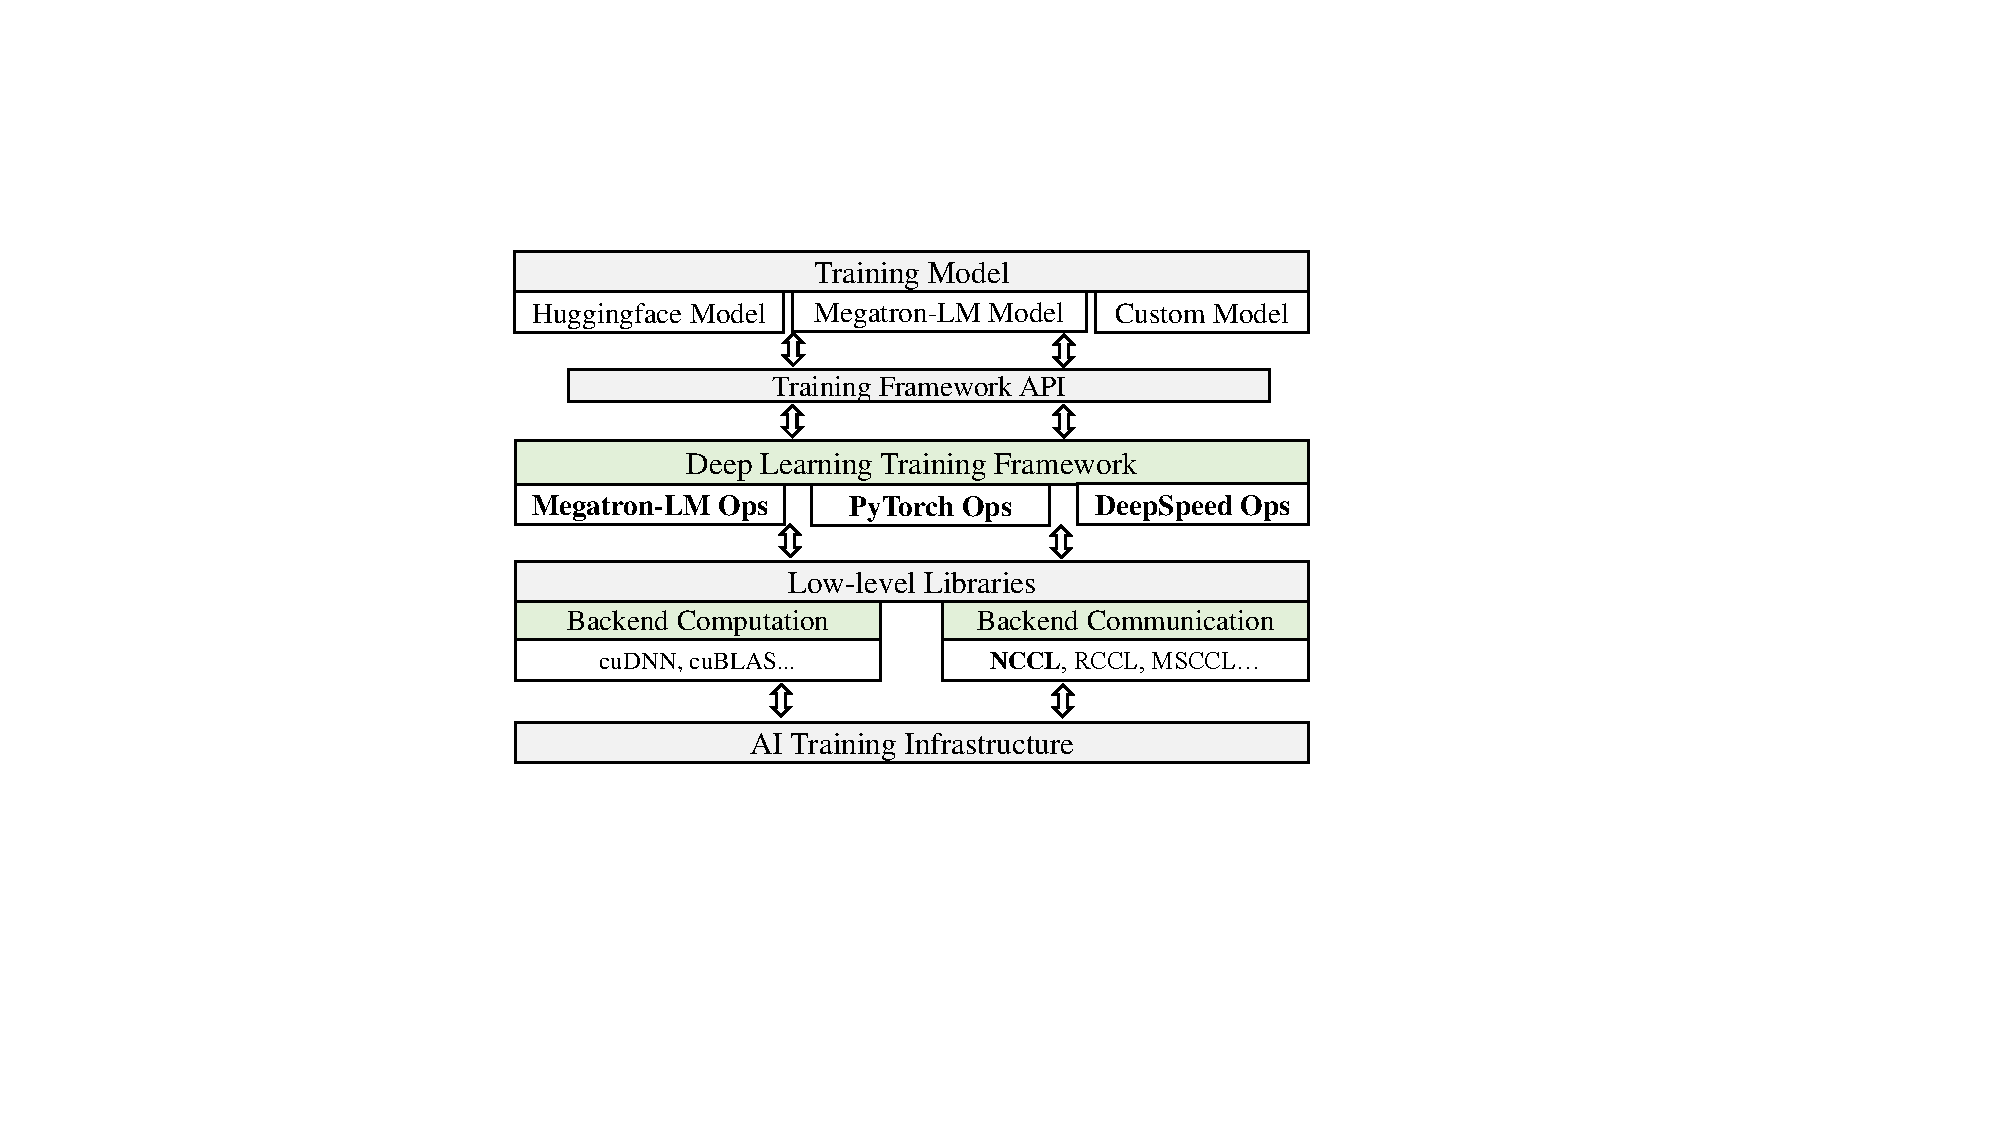
\includegraphics[width=0.9\linewidth]{figures/motivation/tech_overview.pdf} 
    \vspace{-1mm}
    \caption{Overview of the technical stack for LLM training.} 
    \label{fig:tech_overview}
    \vspace{-1.5mm}
\end{figure}
% \noindent\textbf{Training frameworks.} 
LLM training jobs are executed on frameworks such as Megatron-LM~\cite{shoeybi2019megatron} and PyTorch~\cite{rasley2020deepspeed,shoeybi2019megatron,SimAI2025NSDI}. They implement parallelism strategies combining DP, TP, PP, and EP to efficiently scale model training across large GPU clusters. 
Chiefly, DP replicates the model and splits the data, TP divides model parameters among GPUs, PP stages model layers for pipelined execution, while EP distributes experts of a MoE model across devices.
% Together, these methods accelerate training of hundred-billion-parameter models. 
% \noindent\textbf{Communication library.} 
Collective Communication Libraries (CCLs) then facilitate data transfer across ranks. NCCL is the de-facto CCL in production~\cite{weingram2023xccl,shoeybi2019megatron,SimAI2025NSDI,rasley2020deepspeed}.
% , including advanced topological algorithms and protocols that decompose data transmission into efficient P2P transfers.
\begin{table*}[t]
    \centering
    \small
    \setlength{\tabcolsep}{2.5pt}
    \renewcommand{\arraystretch}{0.95}
    \begin{tabular}{@{}cccccccc@{}}
    \toprule

    \multirow{2}{*}[-5pt]{Simulator} & 
    \multicolumn{3}{c}{Training Workload} & 
    \multirow{2}{*}[-5pt]{\makecell{3D Parallelism}} & 
    \multirow{2}{*}[-5pt]{\makecell{MoE/EP \\ Support}} & 
    \multirow{2}{*}[-5pt]{\makecell{Comm. \\ Modeling}} & 
    \multirow{2}{*}[-5pt]{\makecell{Overlap \\ Slowdown}} \\

    \cmidrule(lr){2-4}
    & {\makecell{Framework- \\ Specific Ops}} & {\makecell{Ex-Situ \\ Simulation}} & {\makecell{GPU Memory\\ Simulation}} & & & & \\ 
    \midrule
    FlexFlow~\cite{jia2019beyond} & \xmark & \checkmark & \xmark & \checkmark & \xmark & ${\alpha-\beta}$ model & \xmark \\ 
    Daydream~\cite{zhu2020daydream} & \checkmark & \xmark & \xmark & \xmark & \xmark & ${\alpha-\beta}$ model & \xmark \\
    dPRO~\cite{hu2022dpro} & \checkmark & \xmark & \xmark & \xmark & \xmark & ${\alpha-\beta}$ model & \xmark \\
    DistSim~\cite{lu2023distsim} & \checkmark & \xmark & \xmark & \checkmark & \xmark & ${\alpha-\beta}$ model & \xmark \\ 
    Astra-sim~\cite{won2023astra} & \xmark & -- & \xmark & -- & \xmark & ${\alpha-\beta}$ model & \xmark \\ 
    {Lumos}~\cite{liang2025lumos} & \checkmark & \xmark & \xmark & \checkmark & \xmark & Outsourced & \xmark \\ 
    \fx{TrioSim}~\cite{li2025triosim} & \xmark & \xmark  & \xmark & -- & \xmark & ${\alpha-\beta}$ model & \xmark \\ 
    SimAI~\cite{SimAI2025NSDI} & \checkmark & --  & \xmark & \checkmark & \xmark & Event-driven & \xmark \\ 
    \yc{vTrain}~\cite{bang2024vtrain} & \yc{\xmark} & \yc{\checkmark} & \yc{\xmark} & \yc{\checkmark} & \yc{\xmark} & \yc{${\alpha-\beta}$ model} & \yc{\xmark} \\
    {Calculon}~\cite{isaev2023calculon} & \xmark & \checkmark & Analytical & \checkmark & \xmark & ${\alpha-\beta}$ model & \xmark \\
    Proteus~\cite{duan2024proteus} & \xmark & \checkmark & Analytical & \checkmark & \xmark & ${\alpha-\beta}$ model & -- \\ 
    \textbf{Moye (ours)} & \textbf{\checkmark} & \textbf{\checkmark} & {Ex-Situ Profiling} & \textbf{\checkmark} & \textbf{\checkmark} & White-box & \textbf{\checkmark} \\ 
    \bottomrule
    \end{tabular}
    \caption{
        \yc{Comparison of \sys against existing simulators; \checkmark\ indicates full support, \xmark\ no support, and \textbf{--} partial or conditional support. }
        % Simulators are evaluated on training workload generation (framework-specific operations, ex-situ simulation, dynamic GPU memory footprints), 3D parallelism, MoE architectures (with EP), communication modeling, and handling of overlap-induced slowdowns.
    }
    \label{tab:work_compare}
    \vspace{-1.5em}
\end{table*}


\subsection{Design Goals}

\noindent Our overarching goal is to build a practical simulator for large-scale LLM training.
Specifically, we aim to achieve: 

\begin{itemize}
    % \vspace{-.2em}
    % \item high-fidelity, ex-situ, efficiency, utility
    \item \textbf{High accuracy.} The basic goal is to accurately predict the  end-to-end training step time (\cref{sec:evaluation}). 

    % \vspace{-.2em}
    \item \textbf{\Ep.} 
    If the simulator's input is collected by deploying the job to the target cluster at full scale, i.e. \textit{in-situ} simulation, its utility is fundamentally limited by what is physically available. 
    To be able to explore scales and scenarios beyond what's available, we desire \textit{\ep} design that can simulate a 1k-GPU cluster using a single rank for example (\cref{sec:usecase}).

    \item \textbf{Generality and ease of use.} The simulator should support mainstream training frameworks, model architectures, and parallelism strategies. It should also be easy to use, automating the process as much as possible to minimize manual effort (\cref{subsec:workload_perf}).

    \item \textbf{High efficiency.} The simulator should be fast for large-scale settings to allow efficient exploration of the vast space of training setup (\cref{subsec:overall_perf} and \cref{sec:usecase}).
     

\end{itemize}


\subsection{Design Challenges} 
\label{subsec:challenges}

\noindent Training simulation has attracted attention recently~\cite{SimAI2025NSDI,liang2025lumos,duan2024proteus,won2023astra}.
Inspired by prior work, we also separately consider computation and communication, and computation can be accurately simulated by offline profiling on the target device.
Yet, to achieve the four design goals, there are three key challenges that prior work has not fully addressed.
Table~\ref{tab:work_compare} summarizes existing simulators along these dimensions. %comparison between \sys and existing simulators.  


% Before we discuss the challenges, we note that all experiments in this section are done on a NVIDIA A100 GPU cluster.
% Each 8-GPU node in the cluster has 600 GB/s NVLINK intra-node bandwidth, and four Mellanox ConnectX-6 NICs each with 2x100 Gbps. 
% \fx{Training and bandwidth testing are performed using PyTorch and NCCL-test~\cite{nccltest}, respectively}.% with PyTorch 1.9, NCCL 2.10.3, and CUDA 11.4. 


\vspace{0.3em}
\noindent \textbf{Challenge 1:}
\textit{How to obtain real training workloads on each device without a full-scale deployment?}

Accurate training simulation relies on obtaining the real \textit{training workload} as the foundation.
\textit{Training workload} refers to the execution graph on a target device that encodes the dependencies or execution sequence of computation and communication \ops, plus other necessary information like tensor shapes and data types.
It is the blueprint for replaying the training process on the given device.
In LLM training with complex parallelisms, each device (rank) independently initializes its assigned submodel based on TP, PP, and EP settings, resulting in unique workloads per rank. 
\fx{However, most existing simulators (e.g.,~\cite{SimAI2025NSDI,li2025triosim,duan2024proteus,won2023astra,bang2024vtrain}) do not faithfully support the parallelism strategies commonly used in industrial LLM training, such as the combination of TP, PP, and EP adopted in production systems like DeepSeek-V3~\cite{liu2024deepseek} to scale to thousands of GPUs, and as a result they cannot directly generate realistic per-rank workloads.}

Thus a runtime tracing-based approach is naturally used \cite{hu2022dpro,lu2023distsim,luo2022srifty,zhu2020daydream}: the per-device execution graph is extracted after each device builds its graph in parallel (when the training jobs begins).
This entails a full-scale deployment of the job on the cluster, which severely limits the practical utility of the simulator in large-scale settings.
Some work (Proteus~\cite{duan2024proteus} and Calculon~\cite{isaev2023calculon}) choose to choreograph the per-device training workloads on their own in order to avoid this limitation.
This approach is inherently imprecise since it fails to accurately capture the nuanced runtime characteristics of \textit{framework-specific \ops}---custom or highly optimized \ops based on environment-specific factors (see \cref{subsec:workload_perf}).
\fx{These real workloads are also crucial for accurate GPU memory simulation, while analytical memory models (e.g., \cite{duan2024proteus,isaev2023calculon}) without them can incur up to 2.58$\times$ error in our experiments due to the framework's complex internal memory management and allocation optimizations that are difficult to capture analytically (see \cref{subsec:workload_perf}).}
Therefore how to faithfully capture the training workloads without a full-scale deployment becomes our first challenge.








\vspace{0.3em}
\noindent \textbf{Challenge 2:}
\textit{How to accurately simulate collective communication without high overheads?}

Communication \ops are critical in distributed training, yet hard to simulate as they involve complex interactions among devices and machines, and are affected by a range of network factors such as topology, latency, congestion control, etc. Existing approaches fall into two categories. 
Most simulators like ASTRA-sim~\cite{won2023astra}, FlexFlow~\cite{jia2019beyond}, Calculon~\cite{isaev2023calculon}, Proteus~\cite{duan2024proteus}, and NCCL-Predictor~\cite{nccl} adopt a ${\alpha-\beta}$ model~\cite{valiant1990bridging}, which essentially calculates the running time of a communication \op as $tensor\_size/bandwidth + latency$.
Figure~\ref{fig:bw_compare} shows that the most advanced NCCL-Predictor greatly overestimates the effective bus bandwidth of \ar \ops.
Note NCCL-Predictor already uses additional parameters to account for the impact of hardware, communication protocols (TCP vs RDMA), and algorithms (ring vs tree for \ar), but the over-simplified ${\alpha-\beta}$ model is limited in capturing complex interactions across all these factors.
Moreover, NCCL optimizes communication by integrating hardware offloading and acceleration techniques, such as GPUDirect RDMA~\cite{gdrdma} and GDRCopy~\cite{gdrcopy}, which lead to variations in internal kernel behavior. 
% A communication function consists of numerous concurrent send and receive operations across devices in the process group, each of which incurs overhead.

\begin{figure}[t] 
    \centering 
    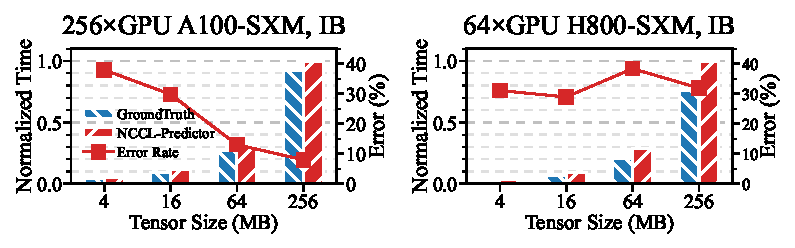
\includegraphics[width=1\linewidth]{figures/motivation/new_motivation_nccl_compare.pdf} 
    \vspace{-5mm}
    \caption{Comparison of predicted communication time (by NCCL-Predictor) and ground truth for \ar.}
    \label{fig:bw_compare} 
    \vspace{-3mm}
\end{figure}

The second, more precise approach involves white-box modeling specifically targeting collective communication (CC) \cite{won2023astra,SimAI2025NSDI}.
Since \nccl (and other CCLs too) implements a CC \op as an orchestrated series of P2P send and receive operations, we can simulate each send and receive to compose the end-to-end result. 
Similar to the training workloads, this naturally reflects the complex optimizations used by CCLs according to topology, NCCL P2P protocol (LL, LL128 or Simple), network interconnect (IB or RoCE), algorithm (ring or tree), etc.
To faithfully simulate the send/receive time, prior work \cite{won2023astra,SimAI2025NSDI} uses packet-level discrete-event network simulators like ns-3 \cite{riley2010ns}, which takes the physical topology and profiled link bandwidth as input.
Yet packet-level simulation is computationally expensive as it needs to simulate the entire protocol stack at each node in the network: 
We run the most recent SimAI \cite{SimAI2025NSDI} with an optimized multi-threaded ns-3, and observe that simulating a single iteration on a 128-GPU cluster takes over 2 hours (7655s) on a 32-core server.
% \fx{
% Extrapolating from this measurement, we find a direct design-space exploration for an 8{,}192-GPU system over 100 training configurations would require on the order of 1.5 years of simulation time (\cref{subsec:overall_perf}).
% In practice, this limits such simulator to a small number of high-fidelity case studies and makes them unsuitable for broad configuration sweeps or rapid training-strategy search (which is a basic ablity requirement for simluators).
% Therefore, the challenge is how to scale white-box communication simulation efficiently—preserving much of the accuracy of these detailed models while avoiding the prohibitive cost of packet-level simulation.
% }
\fx{
Extrapolating from this measurement, a direct design-space exploration for an 8{,}192-GPU system over 100 training configurations would require on the order of 1.5 years of simulation time (\cref{subsec:overall_perf}), effectively confining such packet-level simulators to a small number of high-fidelity case studies and making them unsuitable for systematic configuration sweeps or rapid training-strategy search. 
Thus, our second challenge is how to scale white-box communication simulation efficiently so as to retain much of the accuracy of these detailed models while avoiding the prohibitive cost of packet-level simulation.
}

% \fx{for a 8192 GPUs system design-space exploration over 100 training configurations (cref{}) the time will be 1.5 years. making such approach more suitable for a small number of high-fidelity studies rather than broad configuration sweeps, 非常限制了simulator的功能性。}
% Therefore, the challenge is how to scale the white-box communication simulation efficiently without sacrificing accuracy.


% We denote the slowdown factor to be the ratio between running time profiled with overlapping \ar kernel and the one without \ar kernel.
\vspace{0.3em}
\noindent \textbf{Challenge 3:}
\textit{How to account for the interference between overlapping computation and communication?}


\begin{table}[t]
    \scriptsize
    \centering 
    \resizebox{1\columnwidth}{!}{ 
        \begin{tabular}{@{}lll|ll@{}}
        \toprule
        Model       & Overlapped op & Slowdown & Kernel Type & Slowdown \\ \midrule
        VGG19       & 57.53\% & 37.67\%    & GEMM   & 26.95\%    \\
        GPT2        & 51.75\% & 10.61\%    & Sum    & 50.83\%    \\
        Llama3-8B   & 26.79\% & 7.15\%  & GroupedGEMM  & 11.78\%    \\
        Mixtral-8x7B  & 23.02\%  & 10.55\% & Grad   & 61.37\%    \\ \bottomrule
        \end{tabular}} 
    \caption{Statistics about (1) the proportion of overlapped kernels in different models and the slowdown factors in a training step, and (2) slowdown factors of some common computation \ops. Evaluated with PyTorch (VGG19), DeepSpeed (GPT2), Megatron-LM (Llama3-8B), and Flux~\cite{fluxgithub} (Mixtral-8$\times$7B).
    } 
    \label{table:model_kernel_slowdown} 
    \vspace{-4mm}
\end{table}

Overlapping computation and communication is widely used to improve efficiency and utilization~\cite{jiang2024megascale,chen2024centauri,zhang2017poseidon}.
We find that overlapping introduces non-negligible slowdowns especially to computation \ops, even though they are assigned to separate streams on the GPU.
Here, we define slowdown as the percentage increase in running time when overlapping communication kernels compared to no overlap.\footnote{
{Experiments here are conducted on the NVIDIA A800 cluster described in \cref{subsec:setup}, with software environment aligned to the configuration in~\cref{sec:implementation}.}
}
{
As shown in Table~\ref{table:model_kernel_slowdown}, at least 23\% computation \ops overlap with communication (across training frameworks), leading to a slowdown of up to 1.37x.
}
% Note here \ar as the communication operator overlapping with computation.
We also examine the slowdown to individual kernels.
Table~\ref{table:model_kernel_slowdown} (second column group) shows when overlapped with communication kernels with 25MB messages, running times of common kernels increase by an average of 37.73\%.
The CDF of slowdown factors for all computation kernels of Mixtral-8x7B is presented in Figure~\ref{fig:slowdown_cdf}, where slowdown can reach 800\% with an average of 79.2\%. 
Some recent work~\cite{hwang2023ark} also reported similar slowdowns in production training clusters. 
Despite its salient impact, overlap-induced slowdown has been overlooked by most existing work.
Proteus~\cite{duan2024proteus} uses a simple heuristic factor that varies only with GPU architecture and ML model to account for this slowdown, which is too coarse to be accurate and not generalizable to unseen models.

Simulating the overlap-induced slowdown is a daunting task. 
Ideally, we need to model the kernel-level behavior in order to know exactly how the kernels overlap.
For example, in the widely-used gradient overlap optimization~\cite{zhang2017poseidon}, the simulator must correctly replay the backpropagation computation kernels and schedule communication kernels at precise times to achieve accurate overlap.
Further, for a given computation kernel, its slowdown factor is influenced by various factors of hardware and software setup. 
Table~\ref{table:slowdown_env} shows the slowdown factors of two kernels on different GPUs and CUDA versions vary a lot.
This is because the kernel implementation and resource scheduling ultimately determines how GPU resources are shared and contended among concurrent kernels.
These proprietary details are inaccessible for us, not to mention the complexity of modeling them.
% Thus, how to practically simulate the effect of overlapping computation and communication remains a formidable challenge.


\begin{figure}[t]
    \begin{minipage}{0.26\textwidth}
        \centering 
        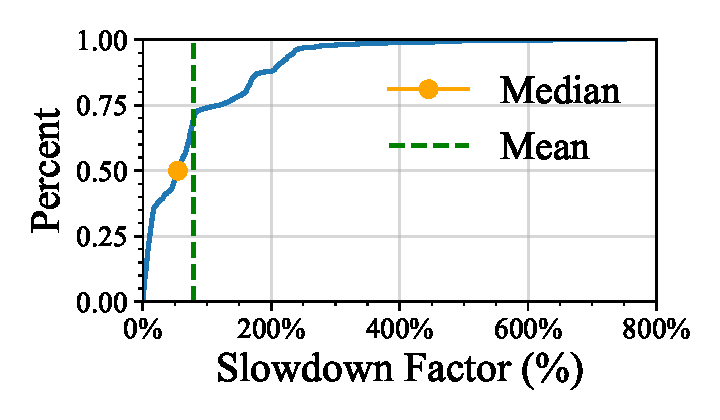
\includegraphics[width=\linewidth]{figures/motivation/slowdown_cdf_positive.pdf} 
        \caption{{CDF of slowdown factor of kernels in Mixtra-8x7B.}} \label{fig:slowdown_cdf} 
    \end{minipage}%
    \hfill
    \begin{minipage}{0.2\textwidth}
        \centering
        \small
        \resizebox{\linewidth}{!}{
            \begin{tabular}{@{}llcccc@{}}
            \toprule
            GPU & Kernel        & CUDA & Slowdown \\ \midrule
            \multirow{4}{*}{\centering 3090}         & GEMM       & 11.8  & 26.4\%     \\
                                                     & GEMM       & 12.1  & 39.3\%      \\
                                                     & LayerNorm  & 11.8  & 18.0\% \\
                                                     & LayerNorm  & 12.1  & 93.8\% \\ \midrule
            \multirow{4}{*}{\centering A800}         & GEMM       & 11.8  & 13.4\% \\
                                                     & GEMM       & 12.1  & 17.8\% \\
                                                     & LayerNorm  & 11.8  & 9.1\% \\
                                                     & LayerNorm  & 12.1  & 20.7\% \\ \bottomrule
            \end{tabular}}
        \captionof{table}{Slowdown of some kernels across GPU architectures and CUDA versions.}
        \label{table:slowdown_env}
    \end{minipage}
    \vspace{-5mm}
\end{figure}

